%fiber_modeling.tex
The first agenda is to determine the Tapered and Lensed Fiber (TLF) model. Because of the heave computing cost creating a full size fiber is not economical. Therefore only the end of the fiber, which provides approximately the equal technical properties, will be modeled in this work. In \cite{TLF_analysis,TLF_mode_transforming} two types of TLF configurations are described.\\ 

\begin{figure}[!ht]
\centering
\subfigure[Tapered cladding TLF.]{
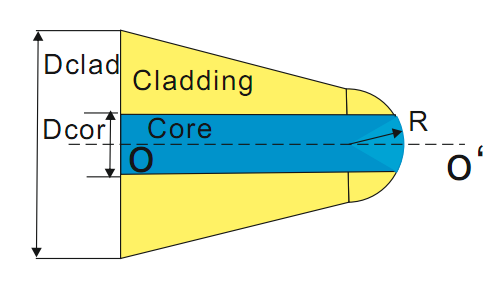
\includegraphics[width=0.4\textwidth]{bilder/lense_fiber_01}
\label{fig:lense_fiber_01}
}
\hfill
\subfigure[Tapered core TLF.]{
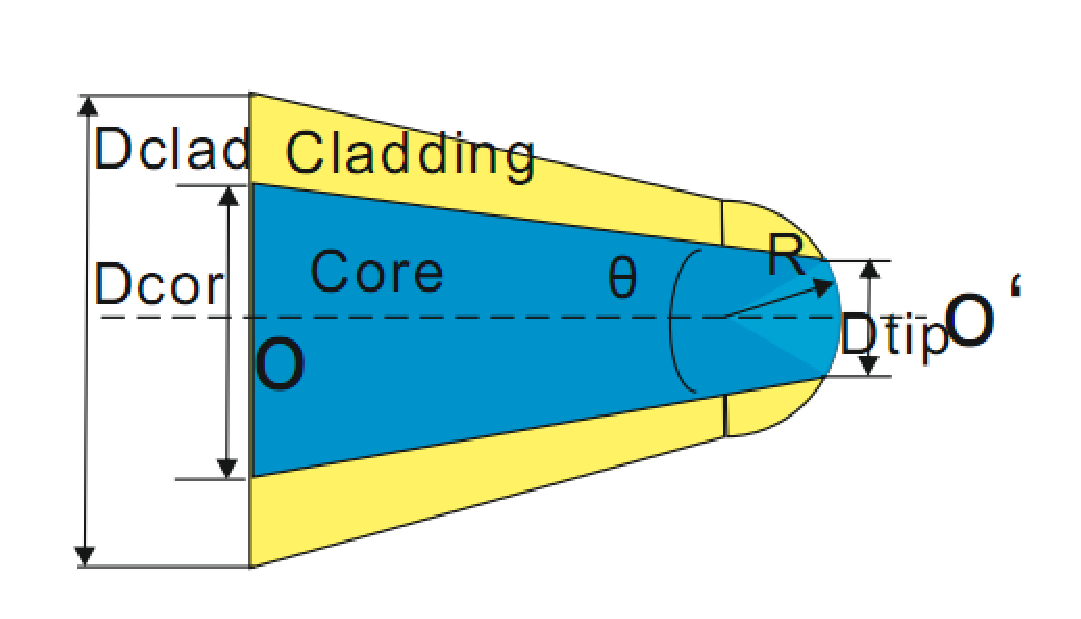
\includegraphics[width=0.4\textwidth]{bilder/lense_fiber_02}
\label{fig:lense_fiber_02}
}
\label{fig:two_TLF}
\caption{Two types of Tapered and Lensed Fibers.}
\end{figure}
The tapered cladding TLF Fig. \ref{fig:lense_fiber_01} shows that its cladding diameter decreases along the propagation direction (O-O' Axis) and the core diameter stays a constant. For the tapered core TLF Fig. \ref{fig:lense_fiber_02} its cladding diameter and core diameter both decrease along the propagation direction. In \cite{TLF_mode_transforming} the Author tried to develop methods to estimate the performance of both type of TLF. Results in \cite{TLF_mode_transforming} show that the performance of the Tapered cladding TLF agrees well with the estimation and that of the Tapered core TLF is unpredictable. In this section two simulation models of each type are created to compare the efficiency of spot size and working distance.\\  

\begin{table}[!ht]
\caption{Configurations of the TLF Models.}
\centering
\begin{tabular}{ccc}
\hline
							&Tapered Cladding&Tapered Core\\
\hline
R($\mu$m) & $6$						 &$6$	\\
n$_{core}$&$1.68$&$1.68$\\
n$_{cladding}$&$1.66$&$1.66$\\
D$_{clad}$($\mu$m) &	$17$ &	$17$\\
D$_{core}$($\mu$m) & $10$ &	$10$\\
D$_{tip}$ ($\mu$m) & --   &	$6$\\
\hline
\end{tabular}
\label{tab:model_fiber_configuration}
\end{table}
First of all, determination the lens of both types is the primary work. In order to simplify the lens structure, a hemispherical lens is assumed at the end of the fiber. Referring to the working distance of the experimental TLF, the lens configuration can be estimated through lens theory. Combining calculations in Matlab and simulations in CST MWS, one configuration of the parameters of the lens can be carefully selected. Tab. \ref{tab:model_fiber_configuration} summarizes the closest parameters for the TLF designs in this work.\\   

With the parameters in Tab. \ref{tab:model_fiber_configuration} the minimum spot location can be estimated. Fig. \ref{fig:lens_spot} demonstrates the beam propagation from the lens based on lens theory. As in previous section \ref{sect:background_optics} described, the minimum spot not exactly locates at coordinate calculated through the focal length. From measurements of the location of Paraxial focal plane (PP) and that of meridional plane (MP) the location of the minimum spot (MS) can be estimated. In the above configuration the theoretical distance from lens end to PP is $8.82 \mu$m and the distance from the lens end to MP is about $2.74 \mu$m. Backward $3/4$ longitudinal spherical aberration (LAm) form PP, the MS is found at the place about $4.26 \mu$m from the lens end. \\ 

\begin{figure}[!ht]
\centering
	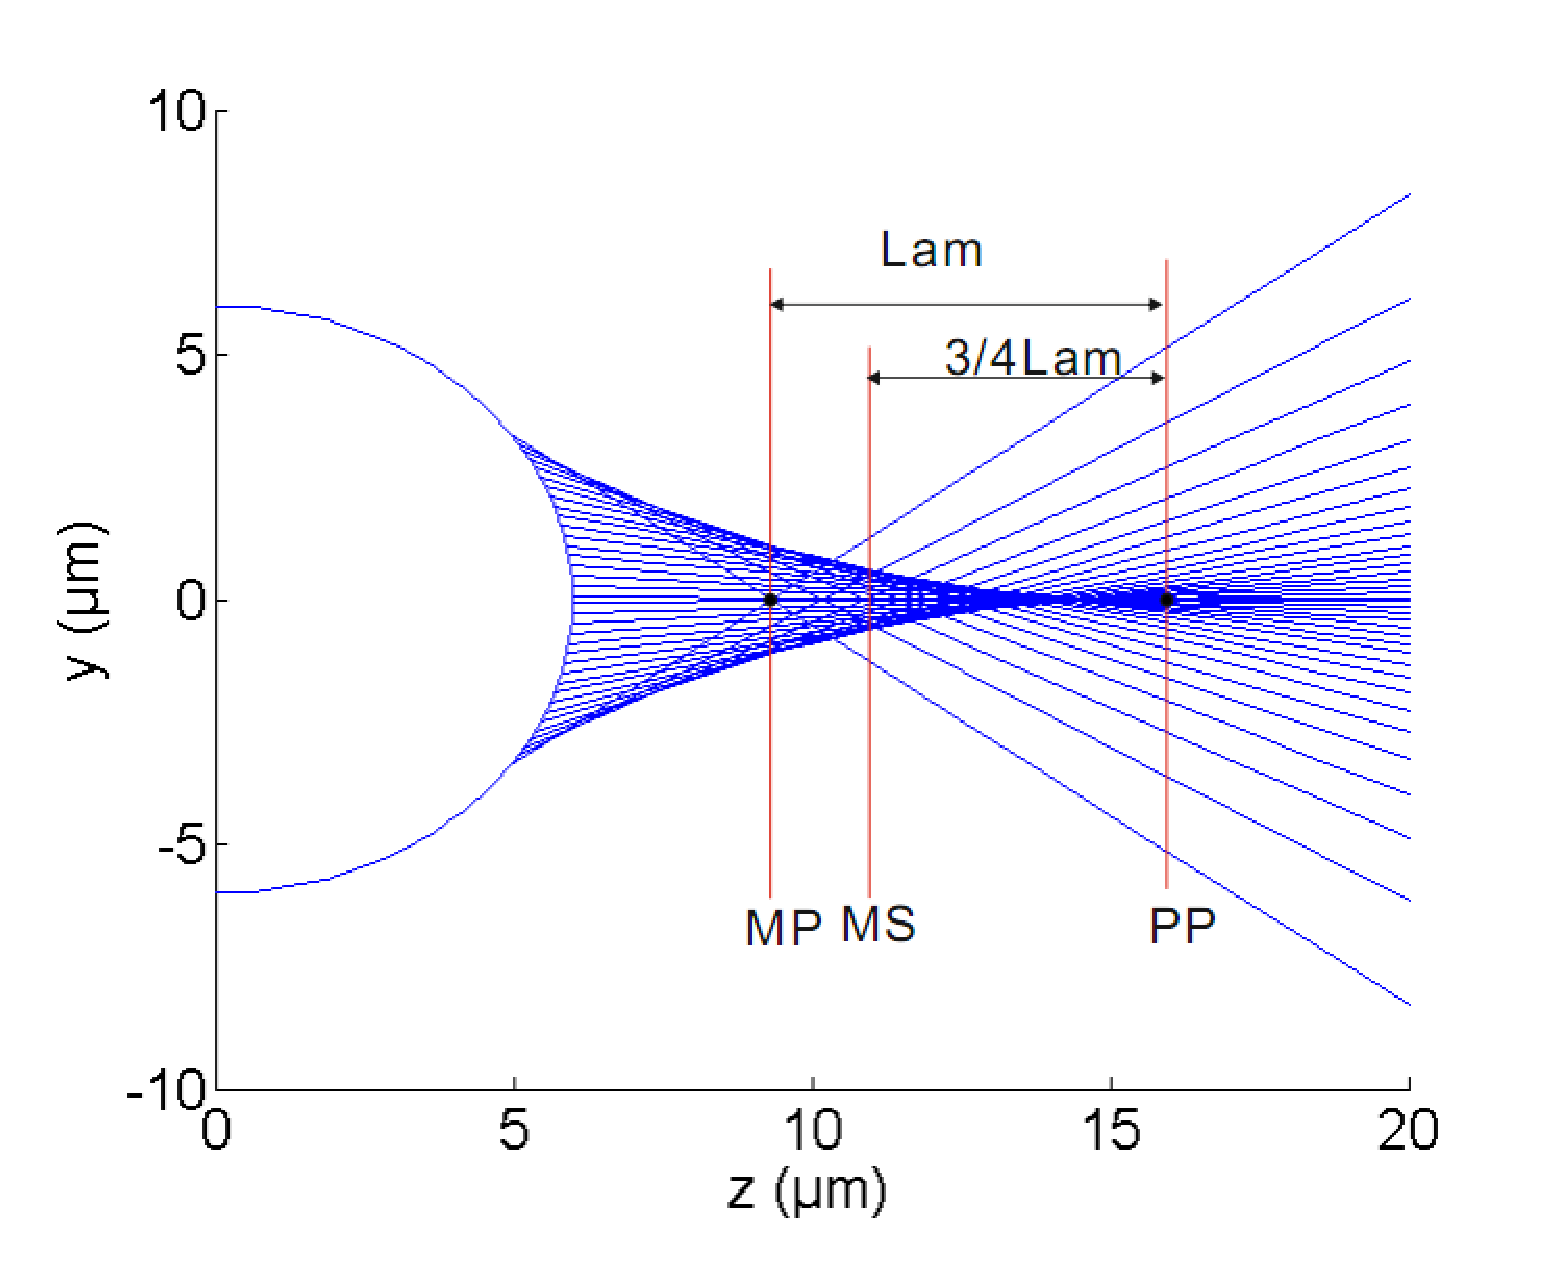
\includegraphics[width=0.7\textwidth]{bilder/cal_min_spot}
\caption{Beam Propogation from lens.}
\label{fig:lens_spot}
\end{figure}
\begin{figure}[!ht]
	\centering
		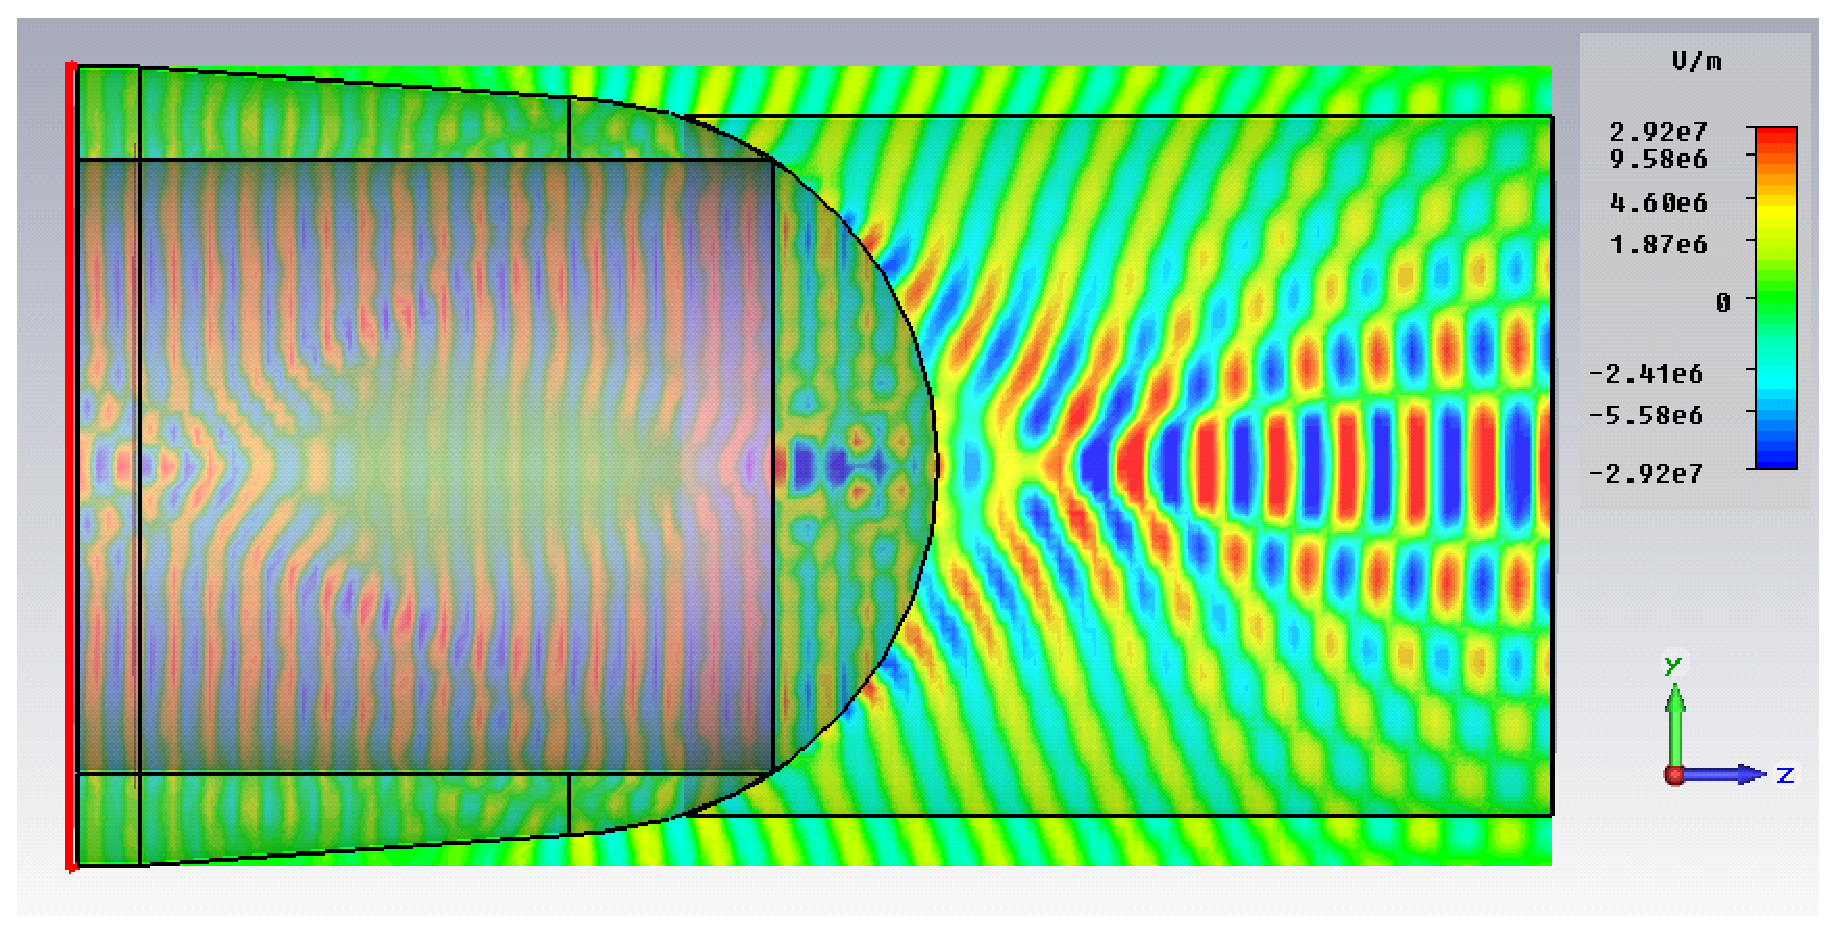
\includegraphics[width=0.7 \textwidth]{bilder/cst_lensed_fiber_equ_efield}
		\caption{E-Field demonstration in logarithmic scale of Tapered cladding TLF.}
 		\label{fig:Tapered_cladding_efield}
\end{figure}

\begin{figure}[!ht]
	\centering
		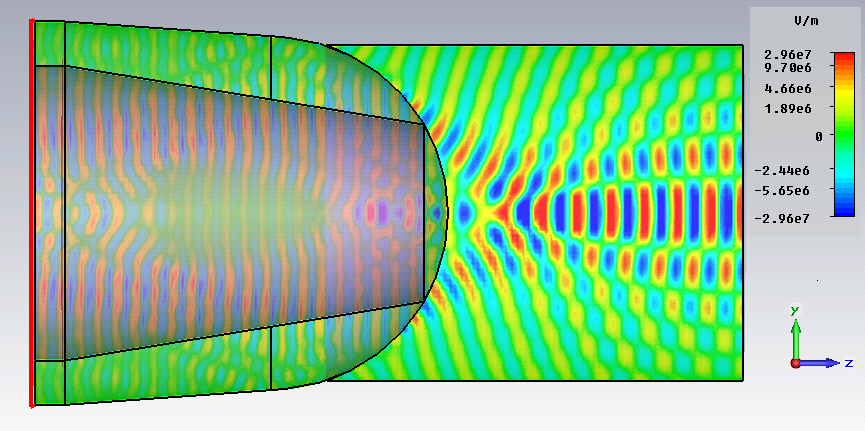
\includegraphics[width=0.7 \textwidth]{bilder/cst_lensed_fiber_efield}
		\caption{E-Field demonstration in logarithmic scale of Tapered core TLF.}
 		\label{fig:Tapered_core_efield}	
\end{figure}
Above only the theoretical working distance of the lens is  estimated. To determine the actual working distance and actual spot size we have to analyze the simulation results from CST MWS. Fig. \ref{fig:Tapered_cladding_efield} and Fig. \ref{fig:Tapered_core_efield} show  E-Field demonstrations  in logarithmic scale in the xz-plane of both types of TLFs. E-Field in both figure are concentrated along the optic axis. We load the power flow data into matlab workspace and draw Fig. \ref{fig:Tapered_cladding_spot_curve} and Fig. \ref{fig:Tapered_core_spot_curve} (seeing Appendix. \ref{app:spot_size}), which show the beam spot diameters through their absolute beam power flow density or its z-compents (propagation direction) of the beam power flow density along the propagation distance. It is obvious that curves of the absolute value of their power flow density indicate the location of the minimum spot more clearly and their values also agree with the previous theoretical location of the minimum spot of lenses. This guess will also be verified in section \ref{sect:optim_shift}. In Fig. \ref{fig:Tapered_cladding_spot_curve} that the minimum spot size locate at about $4.1 \mu$m from lense end and spot size equal about $1.5 \mu$m, while in Fig. \ref{fig:Tapered_core_spot_curve} that the minimum spot size is found at  $4.3 \mu m$ from lense end and spot size equal about $1.5 \mu$m. Thus output properties of both configurations have only small differences. Comparing with the properties given by experimental setup: minimum spot diameter $0.6<d<1.7 \mu$m and working distance $4\mu$m, both TLF models can be acceptable for the following development. In this work the tapered core TLF will be used for further simulations.\\
\begin{figure}[!ht]
		\centering
		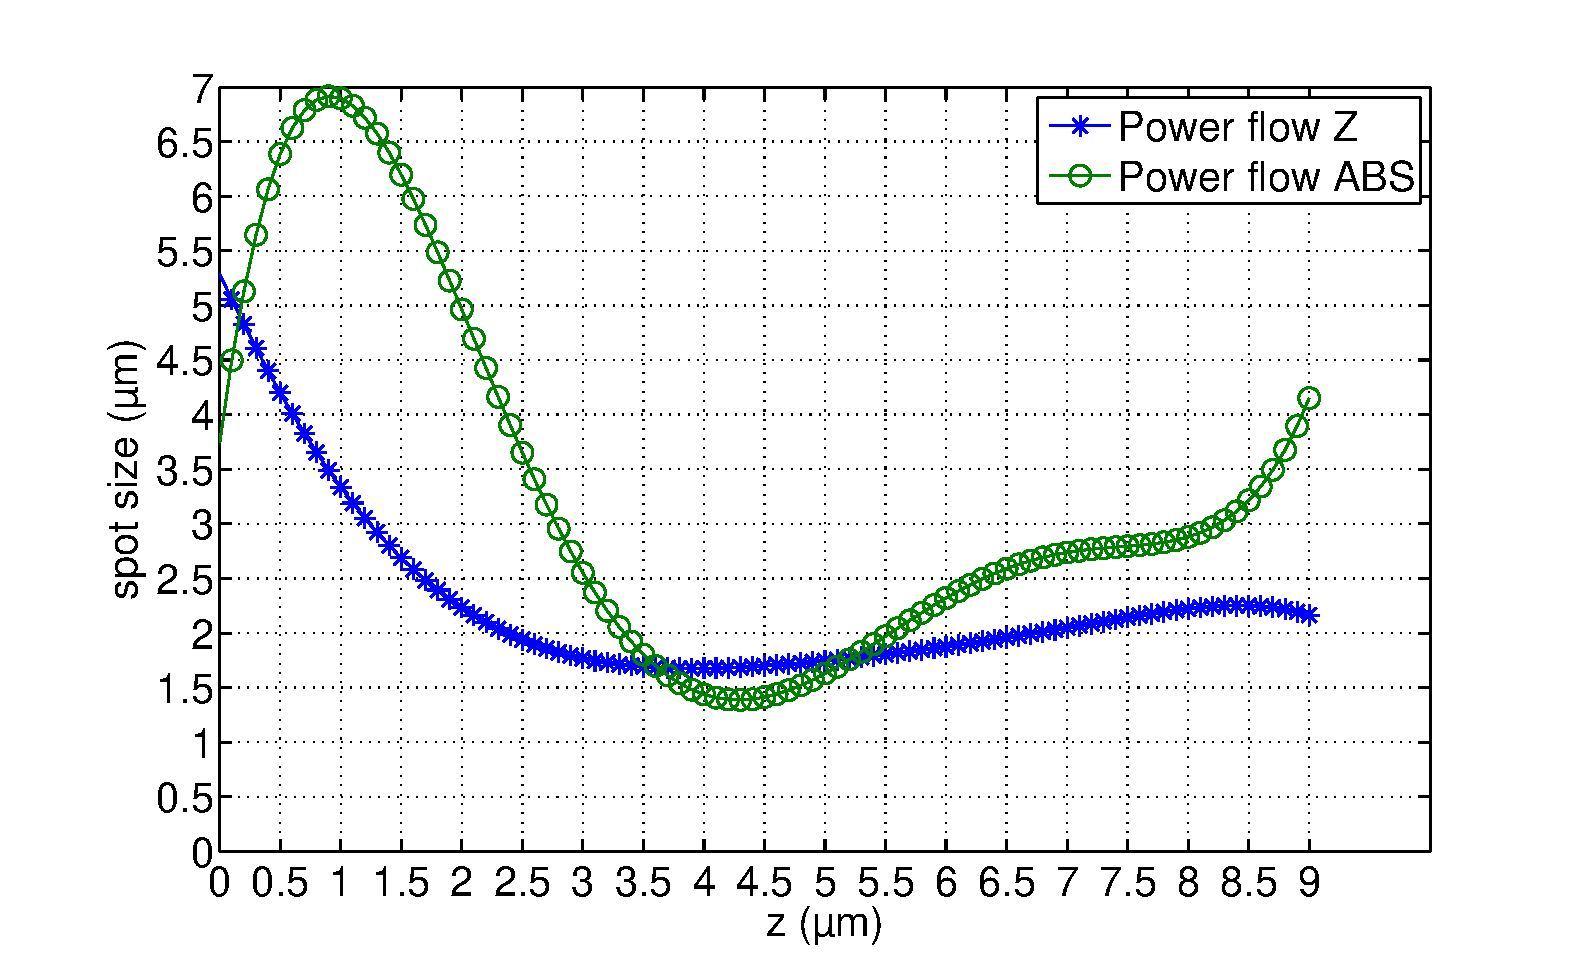
\includegraphics[width=0.7 \textwidth]{bilder/Tapered_cladding_spot_curve}
		\caption{Spot Size Curve of Tapered cladding TLF.}
		\label{fig:Tapered_cladding_spot_curve}
\end{figure} 
\begin{figure}[!ht]
		\centering
		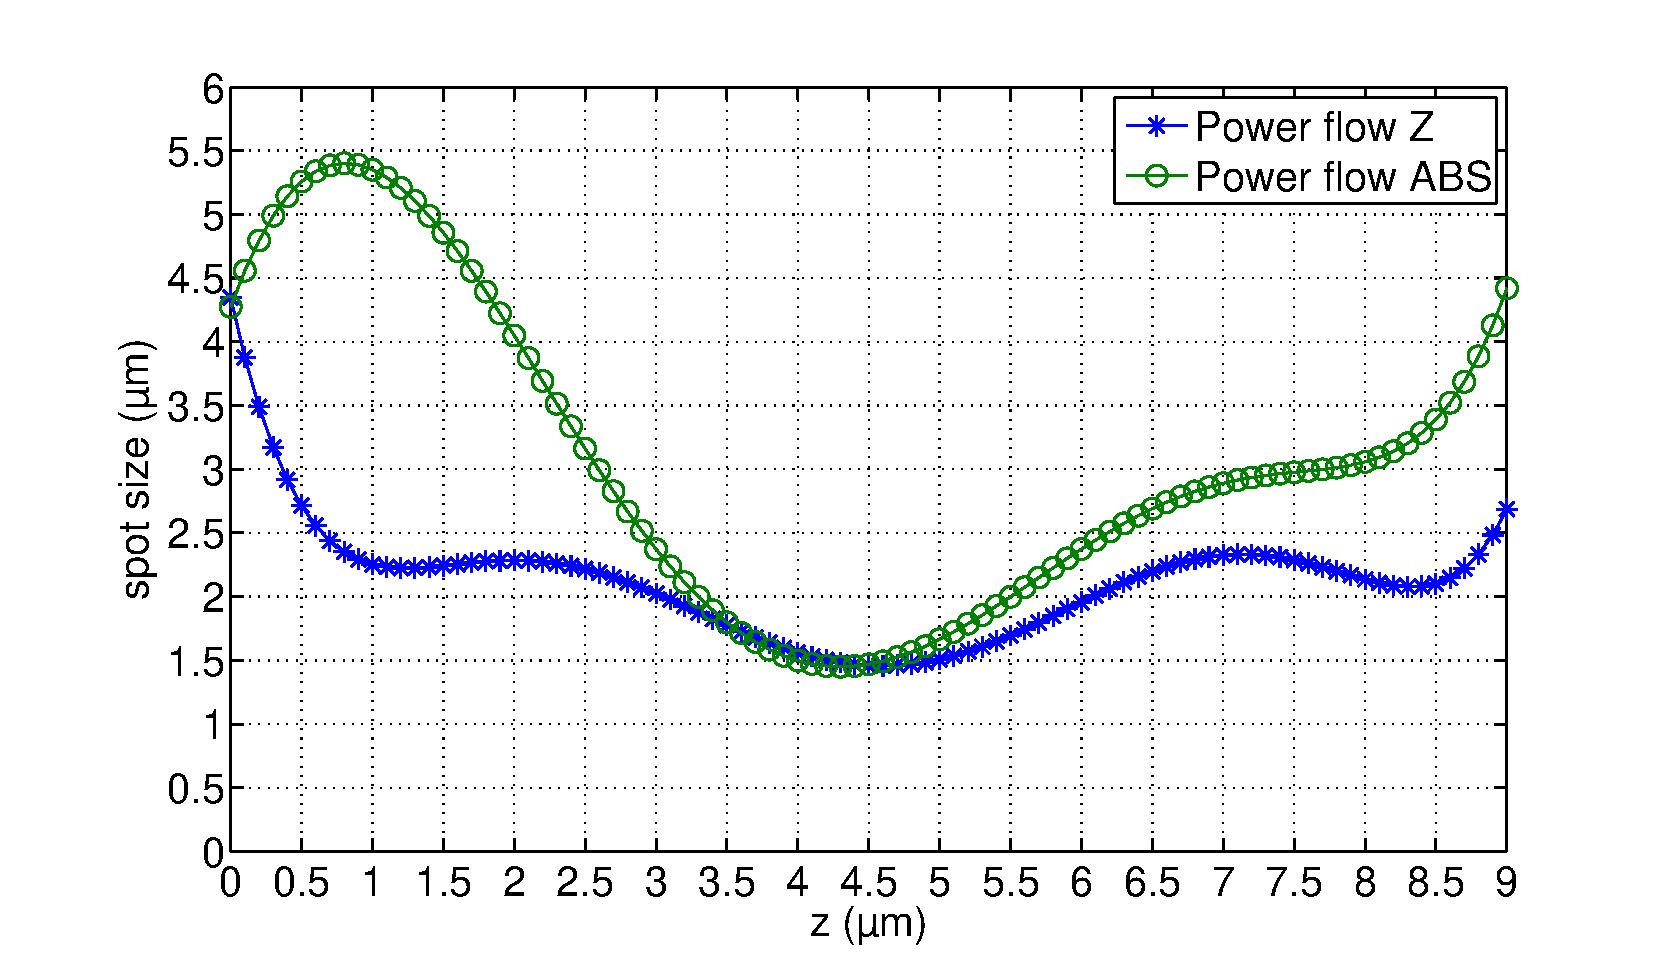
\includegraphics[width=0.7 \textwidth]{bilder/Tapered_core_spot_curve}
		\caption{Spot Size Curve of Tapered core TLF.}
 		\label{fig:Tapered_core_spot_curve}	
\end{figure}
For a more vivid impression of the relation between beam power density and beam propagation distance of the tapered core TLF, 3D Fig. \ref{fig:3d_spot_sub1}-Fig. \ref{fig:3d_spot_sub6} are drawn as demonstrations. It is obvious that the power density of the beam center rises firstly along the distance and at $4\mu$m reaches the highest value. Then it falls slowly. This tendency agrees with the spot size curve inversely. \\
\begin{figure}[!ht]
\centering
\setlength{\abovecaptionskip}{0pt}% 
\flushleft
	\subfigure[3D Beam Power at distance $1\mu m$]{
	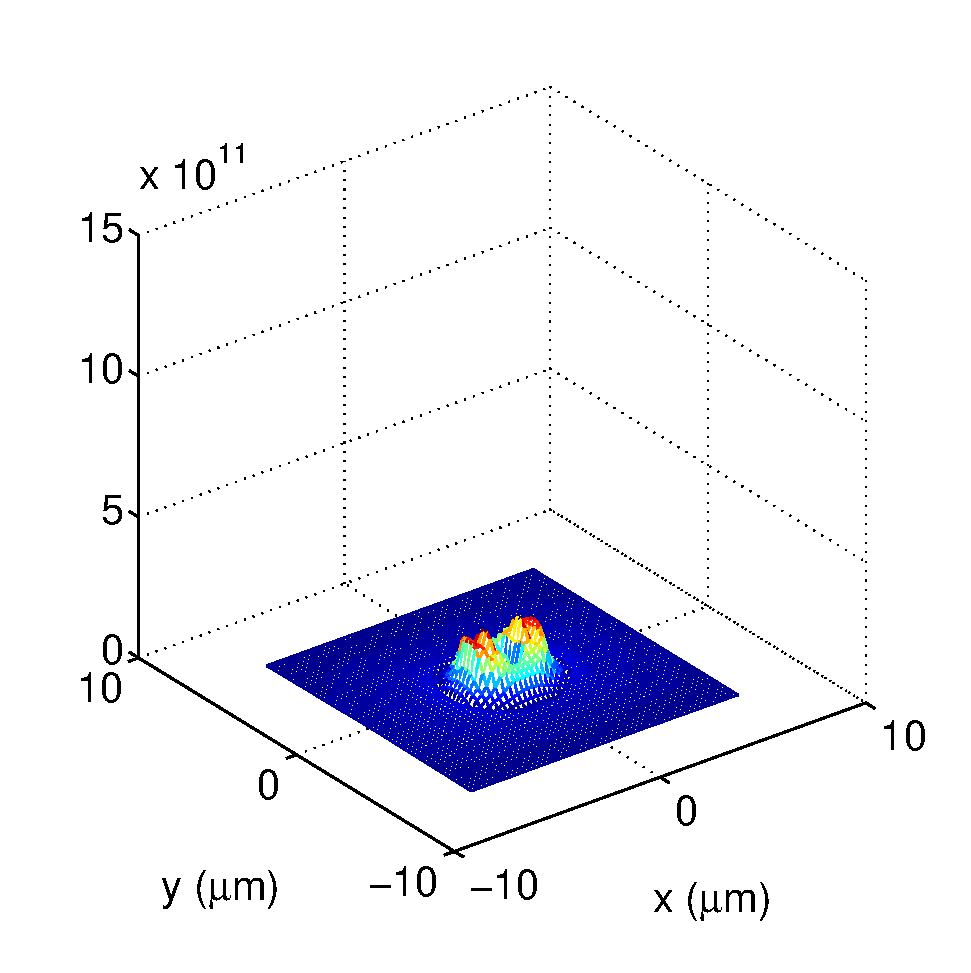
\includegraphics[width=0.37 \textwidth]{bilder/surf_spot_1um}
	\label{fig:3d_spot_sub1}%
	}
	\hfill
 	\subfigure[3D Beam Power at distance $2\mu m$]{
 	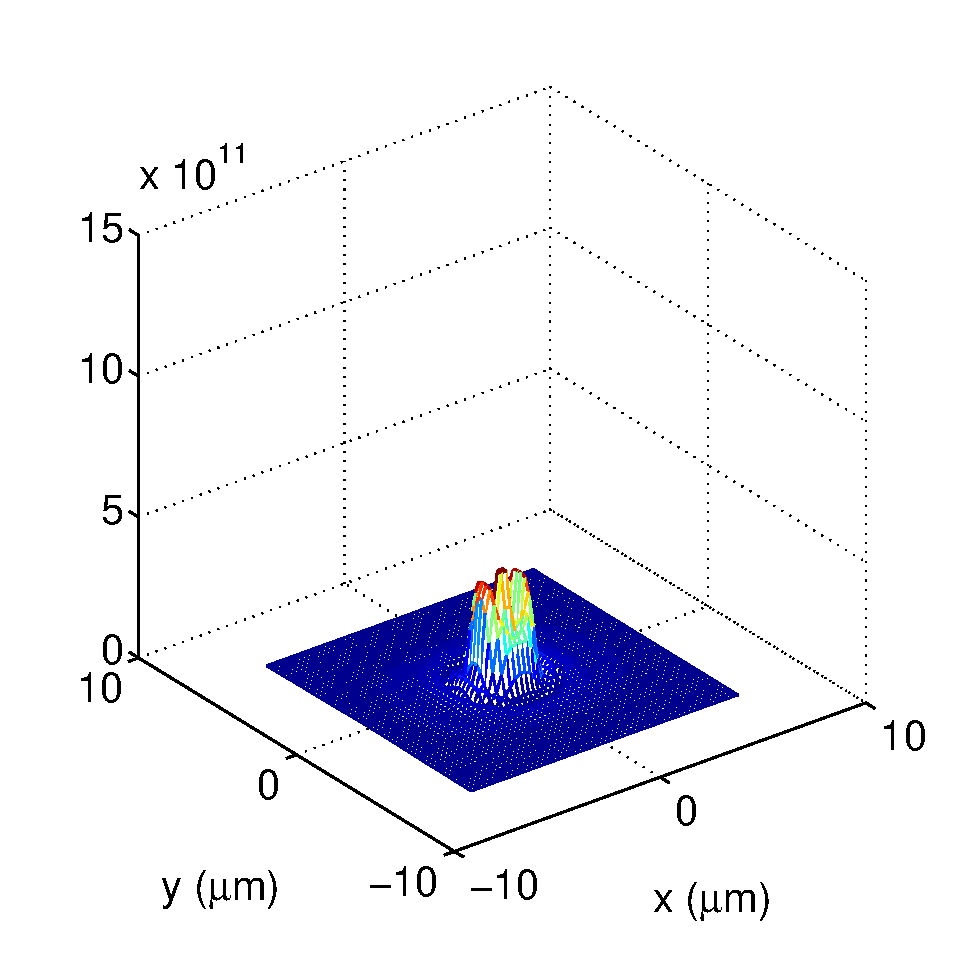
\includegraphics[width=0.37 \textwidth]{bilder/surf_spot_2um}
 	\label{fig:3d_spot_sub2}
 	}
%\end{figure}	
%\begin{figure}[!ht]
%\setlength{\abovecaptionskip}{0pt}% 
%\flushleft
 	 	\subfigure[3D Beam Power at distance $3\mu m$]{
 	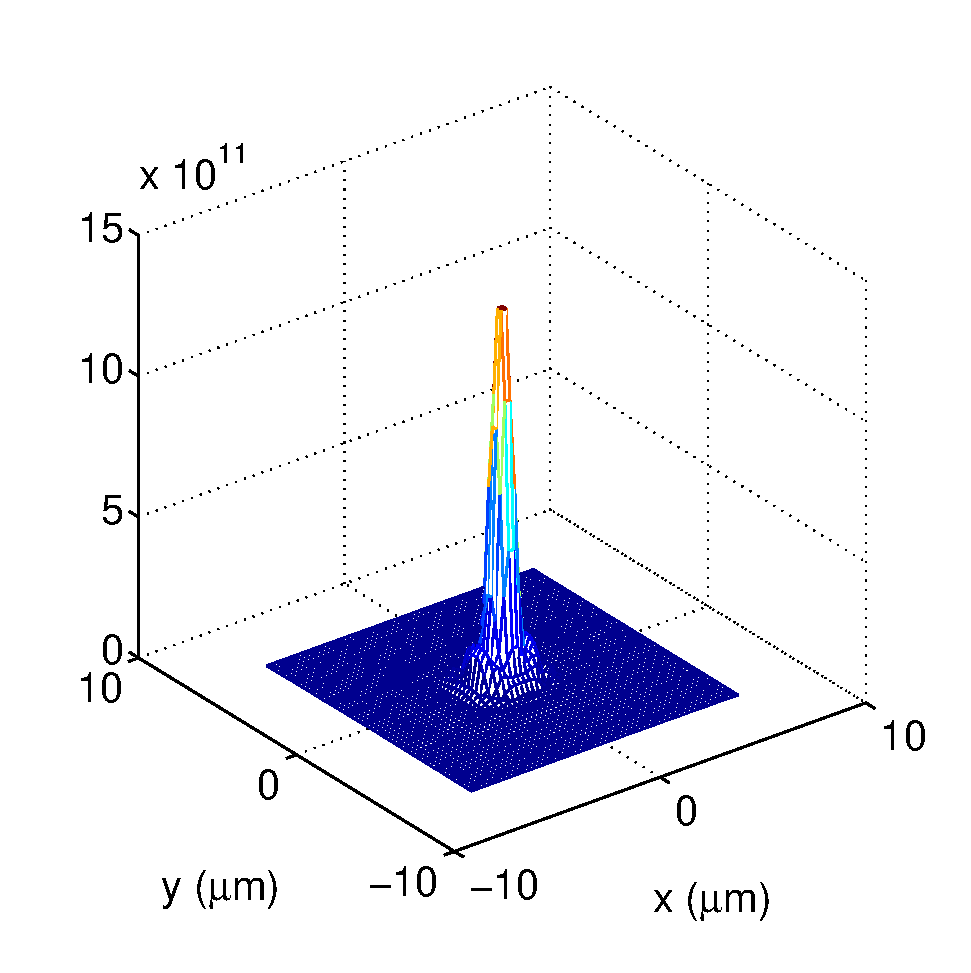
\includegraphics[width=0.37 \textwidth]{bilder/surf_spot_3um}
 	\label{fig:3d_spot_sub3}
 	}
 	\hfill
 	\subfigure[3D Beam Power at distance $4\mu m$]{
 	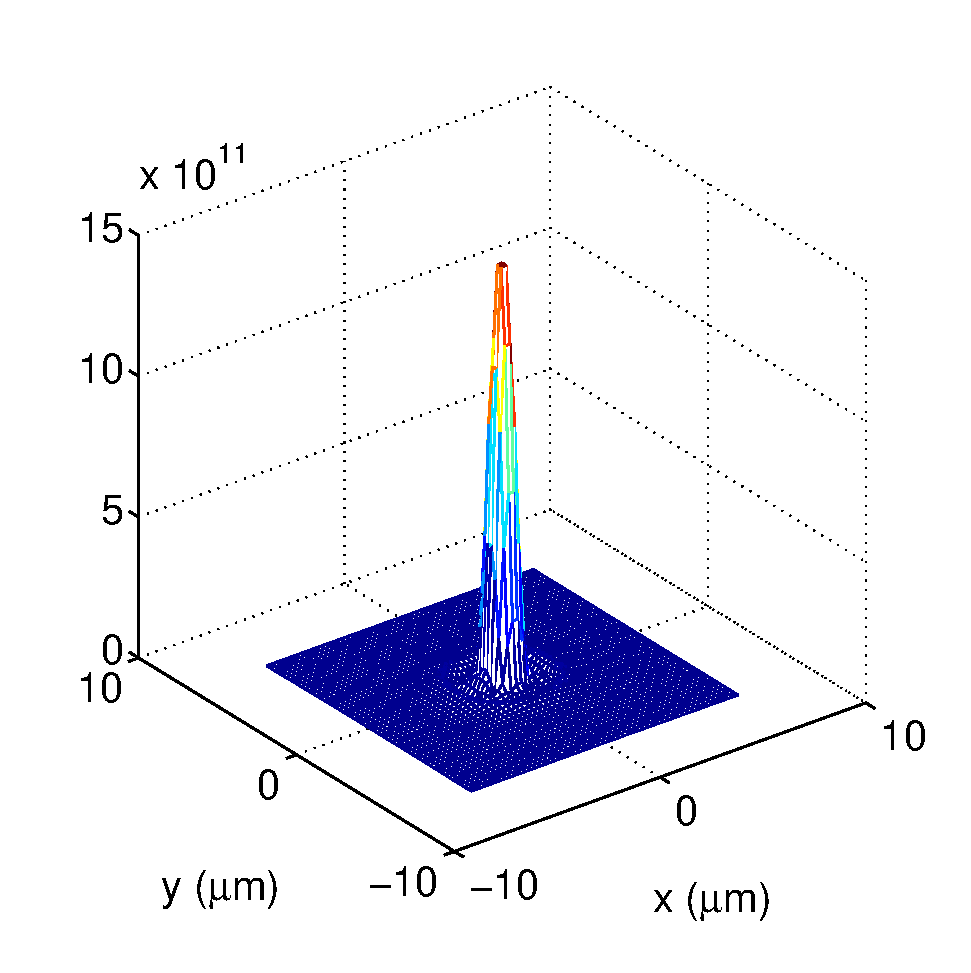
\includegraphics[width=0.37 \textwidth]{bilder/surf_spot_4um}
 	\label{fig:3d_spot_sub4}
 	}
%\end{figure}	
%\begin{figure}[!ht]
%\centering
%\setlength{\abovecaptionskip}{0pt}% 
%\flushleft
 	 \subfigure[3D Beam Power at distance $5\mu m$]{
 	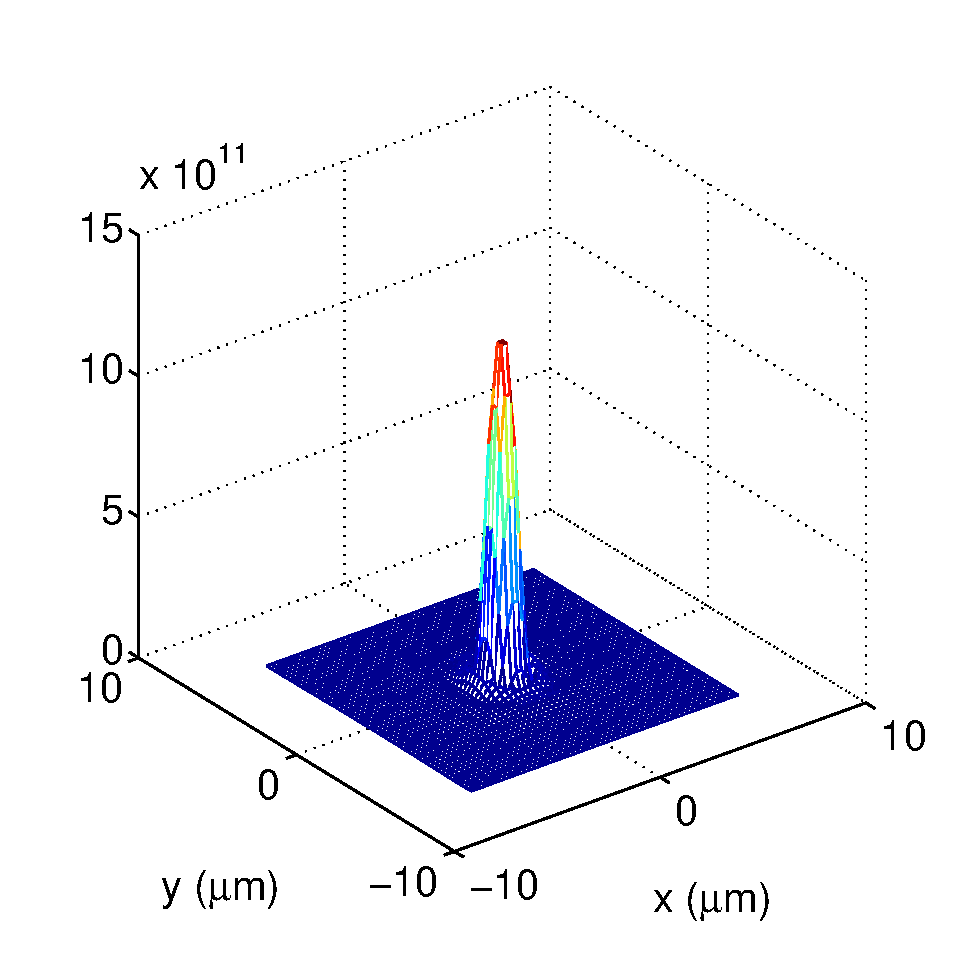
\includegraphics[width=0.37 \textwidth]{bilder/surf_spot_5um}
 	\label{fig:3d_spot_sub5}
 	}
 		\hfill
 	 	\subfigure[3D Beam Power at distance $6\mu m$]{
 	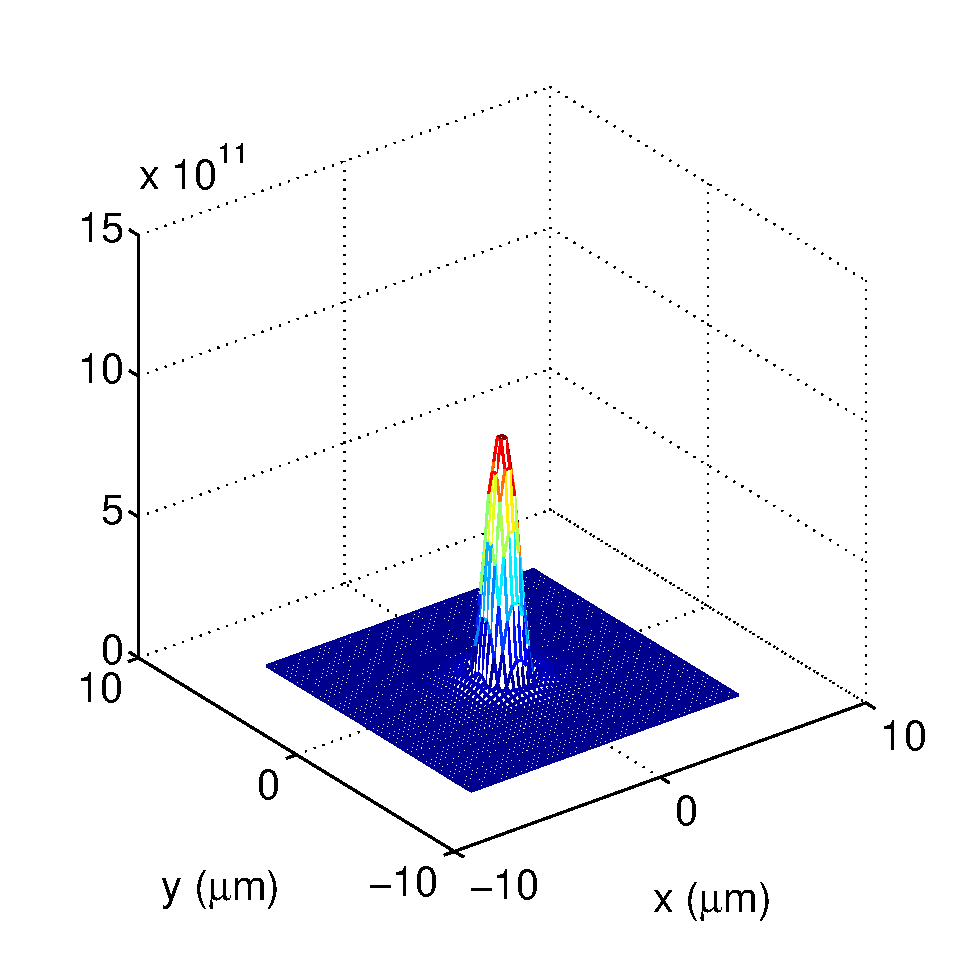
\includegraphics[width=0.37 \textwidth]{bilder/surf_spot_6um}
 	\label{fig:3d_spot_sub6}
 	}
 	\caption{Demonstrations of 3D Beam Power.}
\end{figure}
